\documentclass{standalone}
\usepackage[T1]{fontenc}
\usepackage[latin2]{inputenc}
\usepackage[english]{babel}
\usepackage{tikz}
\usetikzlibrary{calc,through,backgrounds,positioning,fit}
\usetikzlibrary{shapes,arrows,shadows}
 
\begin{document}
 
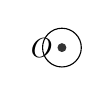
\begin{tikzpicture}[scale=1,inner sep=0.4mm]
\coordinate (O) at (0,0);
\coordinate (A) at (-75:2cm);
\coordinate (B) at (85:2cm);
% ...
\node at (O) [circle,fill=black!80!white] {};
% ...
\draw (0,0) circle (7pt);
\node at (O) [left=2pt] {$O$};
% ...
\end{tikzpicture}
 
\end{document}